% !TeX program = uplatex
\documentclass[a4paper,12pt]{jlreq}

% ===== Packages =====
\usepackage{amsmath,amssymb,mathtools,bm}
\usepackage{siunitx}
\sisetup{detect-all,per-mode=symbol}
\usepackage{physics}
\usepackage{mhchem}
\usepackage{booktabs}
\usepackage{graphicx}
\usepackage{hyperref}
\usepackage{ascmac}
\usepackage{xcolor}


\hypersetup{
  colorlinks=true,
  linkcolor=black,
  urlcolor=blue,
  citecolor=black
}
\usepackage{enumitem}
\usepackage{geometry}
\usepackage{fancybox}
\geometry{margin=25mm}

\begin{document}

\section*{2022年}

以下の問いに答えよ. 結果だけでなく途中の計算も書くこと. 必要に応じて
図を併用してわかりやすい答案にすること. また用いた文字変数の
定義は全て書くこと. 

\subsection*{問2}
半径$a$, 単位長さあたりの巻き数$n$の無限に長いソレノイドコイル
がある.



\begin{figure}[hbtp]
  \centering
  
\includegraphics[width=0.5\linewidth]{images/number3.png} % ← 拡張子・大文字小文字に注意！
  \caption{}
\end{figure}


%%%%%%%%%%%%%%%%%%%%%%%%%%%%%%%%%%%%%%%%
\begin{itembox}[l]{(i)}
  このコイルに一定の電流$I$を流したとき, コイルの中心軸に
作られる磁束密度を求めよ. 大きさだけでなく向きも答えよ. \par
\end{itembox}


\vspace{5mm}

\fbox{解答}\par
半径$a$の無限に長いソレノイドコイルに電流$I$が流れている場合の磁場を
考える. 導線の巻き数は1mあたり$n$回であるとする. 対称性から, 
このソレノイドコイル内外の磁場は, 0でなければ軸に平行で, 大きさは中心軸
からの距離のみに依存する. つまり, 中心軸を$z$軸とする円筒座標系のもとで
\begin{align}
  \bm{H}(\bm{r}) = H(\xi) \bm{e_z}
\end{align}
となる(円形電流が連続的に並んでいると考えると理解できる). 
これを前提に磁場の大きさを求める. \par


\begin{figure}[hbtp]
  \centering
  
\includegraphics[width=0.5\linewidth]{images/number4.png} % ← 拡張子・大文字小文字に注意！
  \caption{}
\end{figure}

図2のように, ソレノイド内部に軸に平行な長さ$l$の辺を持つ任意の長方形
の経路ABCDを考えると, アンペールの法則
\begin{align}
  \oint_C \bm{H}(\bm{r}) \cdot d \bm{r} = \sum_{\text{Cを縁とする任意の面を貫く}}^{} I_i
\end{align}

\begin{align}
  \oint_C \bm{H}(\bm{r}) \cdot d \bm{r} = \sum_{\text{C鎖交する}}^{} I_i
\end{align}

の左辺は
\begin{align}
  \oint_{ABCD} \bm{H}(\bm{r}) \cdot d \bm{r} &= \int_{A}^{B} \bm{H}(\bm{r}) \cdot d \bm{r} + \int_{B}^{C} \bm{H}(\bm{r}) \cdot d \bm{r} + \int_{C}^{D} \bm{H}(\bm{r}) \cdot d \bm{r} + \int_{D}^{A} \bm{H}(\bm{r}) \cdot d \bm{r} \\
  &= \int_{A}^{B} H(\xi_A) \bm{e_z} \cdot dz \bm{e_z} + 0 + \int_{C}^{D} H(\xi_D) \bm{e_z} \cdot (-dz)\bm{e_z} + 0 \\
  &= H(\xi_A) l - H(\xi_D) l
\end{align}
である. 一方, 右辺は電流が面ABCDを貫いていないので0だから
\begin{align}
  &H(\xi_A)l - H(\xi_D)l = 0\\
  &\therefore　 H(\xi_A)l = H(\xi_D)l
\end{align}
となる. 長方形は任意だから, 内部の磁場は$\xi$によらず一定となり
\begin{align}
  H(\xi) = H_{in}　(\xi < a)
\end{align}
である. \par

次に, ソレノイドの外側に, 軸に平行な長さ$l$の辺を持つ長方形の経路A'B'C'D'
を考えると, 上と同様の議論により, 外側の磁場も$\xi$によらず一定となり
\begin{align}
  H(\xi) = H_{out}　(\xi > a)
\end{align}
となる. これは, 長方形が軸から離れる無限遠でも磁場の強さは$H_{out}$である
ことを意味しているが, 無限遠では$H(\infty) = 0$のはずだから, 至る所で
\begin{align}
  H(\xi) = 0　(\xi > a)
\end{align}
である必要がある. \par

次に, ソレノイドをまたぐ, 軸に平行な長さ$l$の辺を持つ任意の長方形の経路
A"B"C"D"を考える. (3)の左辺は辺A"B"の部分以外の寄与は0で
\begin{align}
  \oint_{A"B"C"D"} \bm{H}(\bm{r}) \cdot d \bm{r} = \int_{A'}^{B'}  \bm{H}(\bm{r}) \cdot d \bm{r} = H_{in} l
\end{align}
である. 左辺の$d\bm{r}$の向きをこのように決めると, 右辺の面素$d\bm{S}$
は紙面の表から裏へ向かう. 図のソレノイドの電流は, これと同じ向きに流れているので
右辺の符号は正になる. また, ソレノイドの導線がこの長方形を$nl$回貫いて
いることから, 右辺は$nlI>0$に等しい. よって
\begin{align}
  H_{in}l = nlI
\end{align}
だから, 向きも含めて書くと, 内部では
\begin{align}
  \bm{H}(\bm{r}) = nI\bm{e_z},　\bm{B}(\bm{r}) = \mu nI\bm{e_z}
\end{align}
である. 


%%%%%%%%%%%%%%%%%%%%%%%%%%%%%%%%%%%%%%%%





\vspace{10mm}
%%%%%%%%%%%%%%%%%%%%%%%%%%%%%%%%%%%%%%%%

\begin{itembox}[l]{(ii)}
 中心軸以外での磁場はどうなっているか. コイルの内部, 外部
それぞれについて答えよ. 
\end{itembox}


\vspace{100mm}

\fbox{解答}\par
(i)で述べたように, コイルの内部($\xi < a$)では磁場はどこでも一様で, 
向きは軸方向となり
\begin{align}
  \bm{H}(\bm{r}) = nI\bm{e_z},　\bm{B}(\bm{r}) = \mu nI\bm{e_z}
\end{align}
で, 中心軸だけでなくソレノイド内部の全ての領域で磁場は同じである. 


コイルの外部($\xi > a$)では
\begin{align}
  \bm{H}(\bm{r}) = 0,　\bm{B}(\bm{r}) = 0
\end{align}
である. 



%%%%%%%%%%%%%%%%%%%%%%%%%%%%%%%%%%%%%%%%
\vspace{10mm}

\begin{itembox}[l]{(iii)}
 このコイルの中で電子はどのような運動をするか.
\end{itembox}
\fbox{解答}\par

電場がないとすると, ソレノイド内部では磁場$\bm{B}$は軸方向に一様一定なので
電子(電荷$= -e$)はローレンツ力
\begin{align}
  \bm{F} = -e\bm{v} \times \bm{B}
\end{align}
を受ける. 電子にかかる力が速度$\bm{v}$に常に垂直であるから
\begin{align}
  \bm{F} \cdot \bm{v} = 0
\end{align}
で電子の速度は変化せず, 向きだけが変わる. そこで, 速度を磁場$B$に対して
平行な成分と垂直な成分に分けて考えると, $\bm{v}_{平行}$ではローレンツ力が
働かず等速直線運動をし, $\bm{v}_{垂直}$のもとでは常に速度に垂直な
ローレンツ力が働くから等速円運動をする. よって, 電子の運動は中心軸に沿った
らせん上の運動となる. \par

運動方程式から電子の運動を調べると, $q = -e$としてローレンツ力は
\begin{align}
  \bm{F} = q\bm{v} \times \bm{B} = (-qBv_y, qBv_x, 0)
\end{align}
であるから, 電子の運動方程式は
\begin{align}
  m\frac{dv_x}{dt} &= -qBv_y,\\
  m\frac{dv_y}{dt} &= qBv_x\\
  m\frac{dv_z}{dt} &= 0
\end{align}
とかける. ここで, 電子の質量を$m$とした. (20)式を時間微分して
\begin{align}
  \frac{d^2 v_x}{dt^2} = -\frac{qB}{m}\frac{dv_y}{dt}
\end{align}
となり, この式に(21)式を代入して
\begin{align}
  \frac{d^2 v_x}{dt^2} = -\left(\frac{qB}{m}\right)^2 v_x.
\end{align}
ここで, $\omega = \frac{qB}{m}$とすると, 一般解は$A$と$\alpha$を
任意の定数として
\begin{align}
  v_x = A\sin (\omega t + \alpha)
\end{align}
とかける. (20)式に(25)の一般解を代入すると
\begin{align}
  v_y = -\frac{m}{qB} \frac{dv_x}{dt} = -A \cos (\omega t + \alpha)
\end{align}
を得る. また, 
\begin{align}
  v_z (t) = v_{z0}.
\end{align}
速度の一般解をそれぞれ時間積分して
\begin{align}
  x(t) = \int A\sin(\omega t + \alpha)dt = -\frac{A}{\omega} \cos (\omega t + \alpha) + C_x
\end{align}

\begin{align}
  y(t) = \int (-A\cos (\omega t + \alpha))dt = -\frac{A}{\omega} \sin (\omega t + \alpha) + C_y
\end{align}

\begin{align}
  z(t) = \int v_{z0}dt = v_{z0}t + C_z
\end{align}

(28),(29)より
\begin{align}
  (x - C_x)^2 + (y - C_y)^2 = \left(\frac{A}{\omega}\right)^2
\end{align}
となり, $xy$平面で半径$\frac{A}{\omega}$の円運動をすることがわかる. 
また, 常に中心軸上方向に等速度$v_{z0}$で進むので, ソレノイド内で電子は
らせん運動をする. 



%%%%%%%%%%%%%%%%%%%%%%%%%%%%%%%%%%%%%%%%
\vspace{10mm}

\vspace{100mm}

\begin{itembox}[l]{(iv)}
  磁場は電子に対して仕事をするか.
\end{itembox}


\fbox{解答}\par

ローレンツ力$\bm{F} = q\bm{v} \times \bm{B}$は常に速度$\bm{v}$
と直交しているので, 磁場は電子に対して仕事をしない. 

単位時間あたりの仕事(仕事率)は
\begin{align}
  \frac {dW}{dt} = \bm{F} \cdot \bm{v} = q(\bm{v} \times \bm{B}) \cdot \bm{v} = 0
\end{align}
であるから, 
\begin{align}
  W = \int \bm{F} \cdot d\bm{r} = \int \bm{F} \cdot \bm{v} dt = 0
\end{align}
となる. したがって, 磁場は速度の向きは変化させるが, 速さは変化できず, 
電子に対して仕事をしない. 



%%%%%%%%%%%%%%%%%%%%%%%%%%%%%%%%%%%%%%%%
\vspace{10mm}


\begin{itembox}[l]{(v)}
  このコイルの内部に2枚の平行な平板電極をコイルの中心軸と平行においた. 
中心軸から電極までの距離はともに$d$である. 電極の一方には$V$の電位を, 
もう一方には$-V$の電位を印加した. 平行平板間での電子の運動を議論せよ.
(数式は使わずに, 定性的に記述すれば良い.)
\end{itembox}

\fbox{解答}\par
2枚の平板電極の電位は$+V,-V$なので, 平板間には電位差ができて, 
電場$\bm{E}$が生じる. 電場の向きは, $+V$から$-V$の平板への向きである. 
電子は負の電荷であるから, 電場から受ける力は電場の向きと逆向きで, 
$-V$の平板から$+V$の平板へ力を受ける. また, ソレノイド内では中心軸上むきに
一様な磁場が発生している. 
つまり, ソレノイドコイル内に平行な平板電極を入れると, 
平板間には中心軸に垂直な電場が$+V$から$-V$の平板への向きで生じて, 
電子は負の電荷であるから$-V$の平板から$+V$の平板へ力を受け, 同時に
中心軸上向きの磁場によって横向きにローレンツ力を受けるので, 螺旋状に
運動していき, 最後には$+V$の平板電極へと衝突する. 







%%%%%% コイル図 %%%%%%
\begin{center}

\includegraphics[width=0.5\linewidth]{images/number1.png}
\end{center}

\begin{center}

\includegraphics[width=0.5\linewidth]{images/number2.png}
\end{center}








\vspace{50mm}

\section*{問3}


\begin{itembox}[l]{(i)}
  電気双極子とは何か.
\end{itembox}

\fbox{解答}\par
\begin{center}

\includegraphics[width=0.2\linewidth]{images/number5.png}
\end{center}
(距離$d$は限りなく近い)

図のように, 同じ大きさの正負の電荷$+q$と$-q$の対が距離$d$だけ離れて
存在するとき, 両方をまとめて電気双極子という. $-q$から$+q$に向かう
相対位置ベクトルを$\bm{d}$とするとき
\begin{align}
  \bm{p} = q\bm{d}
\end{align}
を電気双極子モーメントという. $\bm{p}$は$\bm{E}$に比例して
\begin{align}
  \bm{p} = \alpha \epsilon_0 \bm{E}
\end{align}
とかける($\alpha$は分極率という). $\bm{p}$と$\alpha$の次元とSI単位は
\begin{align}
  [\bm{p}] = \text{LQ} : \text{Cm}
\end{align}

\begin{align}
  [\alpha] = [p][\epsilon_0 E]^{-1} = [p][D]^{-1} = \text{QLQ$^{-1}$L$^2$} = \text{L}^3 : \text{m}^3
\end{align}
である. 


\vspace{80mm}
\begin{itembox}[l]{(ii)}
  電気双極子$\bm{p}$が$\bm{r}$だけ離れた地点に作る静電ポテンシャルは
  \begin{align}
    \phi(\bm{r}) = \frac{\bm{p} \cdot \bm{r}}{4\pi \epsilon_0 r^3}
  \end{align}
  と書けることを示せ. 
\end{itembox}


\fbox{解答}\par

電気双極子を結ぶ線分上の中点を原点とし, 電気双極子$+q$と$-q$が
それぞれ$\frac{\bm{d}}{2}, -\frac{\bm{d}}{2}$にあるとすると, 
電気双極子の周りの静電ポテンシャルは, 正負の電荷が作る静電ポテンシャル
の重ね合わせから求められて($d$は微少量なのでOは微小)
\begin{align}
  \phi(\bm{r}) &= \frac{q}{4\pi \epsilon_0 \left|\bm{r} - \frac{\bm{d}}{2}\right|} + \frac{-q}{4\pi \epsilon_0 \left|\bm{r} + \frac{\bm{d}}{2}\right|}\\
  &= 4\pi \epsilon_0 \left(\frac{1}{r\sqrt{1 - \frac{\bm{r \cdot d}}{r^2} + \frac{d^2}{4r^2}}} - \frac{1}{r\sqrt{1 + \frac{\bm{r \cdot d}}{r^2} + \frac{d^2}{4r^2}}}\right)\\
  &= \frac{q}{4\pi \epsilon_0 r} \left\{\left[ 1 + \frac{\bm{r \cdot d}}{2r^2} + O\left(\frac{d}{r}\right)^2\right] - \left[ 1 - \frac{\bm{r \cdot d}}{2r^2} + O\left(\frac{d}{r}\right)^2\right]\right\} \\
  &\approx.  \frac{q}{4\pi \epsilon_0 r} \frac{\bm{r \cdot d}}{r^2} = \frac{\bm{p \cdot r}}{4\pi \epsilon_0 r^3}.
\end{align}




\begin{itembox}[l]{(iii)}
  電場は
  \begin{align}
    \bm{E}(\bm{r}) = \frac{1}{4\pi \epsilon_0} \frac{3(\bm{p \cdot r})\bm{r} - r^2 \bm{p}}{r^5}
  \end{align}
  と書けることを示せ. 
\end{itembox}
\fbox{解答}\par

電気双極子は対称性が高くなく, ガウスの法則で電場を計算できないので, 
\begin{align}
  \bm{E}(\bm{r}) = \sum_{i = 1}^{n}\frac{q_1 q_2}{4\pi \epsilon \left|\bm{r}_2 - \bm{r}_1\right|^2} \bm{e}_{\bm{r}_2 - \bm{r}_1} = \sum_{i = 1}^{n} \frac{q_i (\bm{r} - \bm{r}_i)}{4\pi \epsilon_0 \left|\bm{r} - \bm{r}_i\right|^3}
\end{align}
より, 電気双極子の位置は(ii)と同様にして
\begin{align}
  \bm{E}(\bm{r}) = \frac{q\left(\bm{r} - \frac{\bm{d}}{2}\right)}{4\pi \epsilon_0 \left|\bm{r} - \frac{\bm{d}}{2}\right|^3} + \frac{-q\left(\bm{r} + \frac{\bm{d}}{2}\right)}{4\pi \epsilon_0 \left|\bm{r} + \frac{\bm{d}}{2}\right|^3}
\end{align}
であるが, 
\begin{align}
  \left|\bm{r} \pm \frac{\bm{d}}{2}\right| &= \sqrt{\left(\bm{r} \pm \frac{\bm{d}}{2}\right) \cdot \left(\bm{r} \pm \frac{\bm{d}}{2}\right)} \\
  &= \sqrt{r^2 \pm \bm{r \cdot d} + \frac{d^2}{4}}\\
  &= r\left(1 \pm \frac{\bm{r \cdot d}}{r^2} + \frac{d^2}{4r^2}\right)^{1/2}
\end{align}
だから, 
\begin{align}
  \bm{E}(\bm{r}) = \frac{q\left(\bm{r} - \frac{\bm{d}}{2}\right)}{4\pi \epsilon_0 r^3\left(1 - \frac{\bm{r \cdot d}}{r^2} + \frac{d^2}{4r^2}\right)^{3/2}} + \frac{-q\left(\bm{r} + \frac{\bm{d}}{2}\right)}{4\pi \epsilon_0 r^3\left(1 + \frac{\bm{r \cdot d}}{r^2} + \frac{d^2}{4r^2}\right)^{3/2}}
\end{align}
となる. 電気双極子より十分離れた点, すなわち$|r| >> |\bm{d}|$
である点では, マクローリン級数に展開することで
\begin{align}
  \bm{E}(\bm{r}) &= \frac{q}{4\pi \epsilon_0 r^3} \left\{\left(\bm{r} - \frac{\bm{d}}{2}\right)\left[1 + \frac{3\bm{r \cdot d}}{2r^2} + O\left(\frac{d}{r}\right)^2\right] - \left(\bm{r} + \frac{\bm{d}}{2}\right)\left[1 - \frac{3\bm{r \cdot d}}{2r^2} + O\left(\frac{d}{r}\right)^2\right]\right\}\\
  &\approx \frac{q}{4\pi \epsilon_0 r^3} \left[\frac{3(\bm{r \cdot d})\bm{r}}{r^2} - \bm{d}\right]
\end{align}
とできる. $O\left(\frac{d}{r}\right)^2$は, 2次の微少量を表す. 
(34)式から
\begin{align}
  \bm{E}(\bm{r}) \approx \frac{1}{4\pi \epsilon_0}\left[\frac{3(\bm{p \cdot r})\bm{r}}{r^5} - \frac{\bm{p}}{r^3}\right]
\end{align}
と示せる. 

\begin{align}
  \bm{E}(\bm{r}) = -\text{grad}\phi(\bm{r})
\end{align}
を計算することでも電場の導出を行う. 
%%%%%%%%%%%%%%%%%%%%%%%%%

\newpage


\section*{2023年}




\begin{itembox}[l]{\textbf{問}}
  $xy$平面に無限に広く厚さが無視できる金属板がある. 空欄に入る式や値を答えよ.
  また, (iii)については, 結果だけでなく途中の計算も書くこと. 
\end{itembox}

\begin{itembox}[l]{(i)}
  この金属板に正の一様な電荷を与えた. 電荷密度は単位面積当たり$\rho$であるとする.
  点(0,0,d)における電場を求めよ. 
\end{itembox}
\fbox{解答}\par

金属板を$xy$平面とし, この平面に垂直な方向を$z$軸とすると
電荷分布の対称性から電場は金属板に垂直で$\bm{E} = (0,0,E_z)$と考えられる.
$z$軸を中心軸とし, 上面と下面が平板から同じ距離$a$とする円柱に対して
ガウスの法則を用いる. 電荷分布の対称性から$E_z(a) = -E_z(-a)$であり, 
この円柱の体積を$V$, 表面積を$S$とするとガウスの法則を用いて
\begin{align}
  \int_{S}^{} \bm{E} \cdot d\bm{S} &= \int_{上面}^{} \bm{E} \cdot d\bm{S} + \int_{側面}^{} \bm{E} \cdot d\bm{S} + \int_{下面}^{} \bm{E} \cdot d\bm{S}\\
  &= \int_{V}^{} \frac{\rho}{\epsilon_0}.
\end{align}
円柱の側面で面素ベクトル$d\bm{S}$は電場と垂直になるので, 円柱側面の面積分は
考慮せず
\begin{align}
  \int_{S}^{} \bm{E} \cdot d\bm{S} &= \int_{上面}^{} \bm{E} \cdot d\bm{S} +  \int_{下面}^{} \bm{E} \cdot d\bm{S}\\
  &= \int_{V}^{} \frac{\rho}{\epsilon_0}.
\end{align}
円柱の上面と下面の面積を$S'$とすると(下面で$d\bm{S}$は$-z$軸方向)
\begin{align}
  \int_{上面}^{} \bm{E} \cdot d\bm{S} &= E_z (d)S'\\
  \int_{下面}^{} \bm{E} \cdot d\bm{S} &= -E_z (-d)S'
\end{align}
であるが, 電荷分布の対称性から$E_z(d) = -E_z(-d)$なので
\begin{align}
  &\int_{上面}^{} \bm{E} \cdot d\bm{S} +  \int_{下面}^{} \bm{E} \cdot d\bm{S}\\
  &= E_z (d)S' + (-E_z (-d))S' = 2E_z (d) S'
\end{align}
となるので, ガウスの法則から
\begin{align}
  2E_z (d) S' = \frac{\rho}{\epsilon_0}S'
\end{align}
より
\begin{align}
  E_z (d) = \frac{\rho}{2\epsilon_0}
\end{align}
を得る. よって, 金属板の上下で
\begin{align}
  E_z = \begin{cases}
    \frac{\sigma}{2\epsilon_0} & (z>0),\\
    -\frac{\sigma}{2\epsilon_0} & (z<0)
  \end{cases}
\end{align}
となる. 

\vspace{20mm}


\begin{itembox}[l]{(ii)}
  この金属板を接地して, 点(0,0,d)に点電荷$q$を置いた. 
  電荷$q$が受ける力を求め, また金属板に誘起される電荷分布を求めよ. 
  加えて, これを金属板上で積分するとどうなるか？
\end{itembox}
\fbox{解答}\par

はじめに, 電荷$q$が受ける力を求める. 金属板を跨いで点(0,0,-d)に点電荷$-q$
があると仮定する. このとき, 点(0,0,d)にある点電荷$q$が受ける力は
\begin{align}
  \bm{F} &= \frac{q \cdot (-q)}{4\pi \epsilon_0 \cdot (2d)^2} \bm{e}_z\\
  &= -\frac{q^2}{16\pi \epsilon_0 d^2} \bm{e}_z.
\end{align}

また, 金属板に誘起される電荷分布は電気双極子モーメント$\bm{d} = 2d\bm{e}_z$
を考えて($r = \sqrt{x^2+y^2+z^2}$)
\begin{align}
  \bm{E}(\bm{r}) &= \frac{q(\bm{r} - d\bm{e}_z)}{4\pi \epsilon_0 |\bm{r} - d\bm{e}_z|^3} + \frac{q(\bm{r} + d\bm{e}_z)}{4\pi \epsilon_0 |\bm{r} + d\bm{e}_z|^3}\\
  &= \frac{q(\bm{r} - d\bm{e}_z)}{4\pi \epsilon_0 (r^2 - 2dz + d^2)^{3/2}} - \frac{q(\bm{r} + d\bm{e}_z)}{4\pi \epsilon_0 (r^2 + 2dz + d^2)^{3/2}}
\end{align}
金属板の限りなく近いところでの電場は, 円筒座標$(\xi,\phi,z)$を用いて
\begin{align}
  z \approx 0,　r \approx \xi
\end{align}
であるから
\begin{align}
  \bm{E}(\bm{\xi}) = \frac{-dq}{2\pi \epsilon_0 (\xi^2 + d^2)^{3/2}}\bm{e}_z.
\end{align}
(i)のように, 円筒についてガウスの法則を適用すると
\begin{align}
  \int \bm{E} \cdot d\bm{S} = \int_{V}^{} \frac{\rho}{\epsilon_0}
\end{align}
において左辺は円筒の上面下面の微小面積を$S''$とし, 
\begin{align}
  (左辺) = E_z(d)S''
\end{align}
である. 右辺については, 円筒内部に含まれる金属板表面の電荷なので
\begin{align}
  (右辺) \approx \rho(\bm{r})S''
\end{align}
である. よって, 
\begin{align}
  E(\bm{r}) \approx \frac{\rho(\bm{r})}{\epsilon_0}
\end{align}
微小面積を限りなく0に近づけ, かつ金属板表面に$\bm{r}$を限りなく近づけて
電場の向きは表面の法線ベクトル$\bm{n}(\bm{r}) = \bm{e}_z$に平行であるから
\begin{align}
  \frac{-dq}{2\pi \epsilon_0 (\xi^2 + d^2)^{3/2}}\bm{e}_z = \frac{\rho(\bm{r})}{\epsilon_0}\bm{e}_z
\end{align}
より
\begin{align}
  \rho (\bm{r}) = \frac{-dq}{2\pi (\xi^2 + d^2)^{3/2}}
\end{align}
と求められる. 

これを金属板上で積分すると, 
\begin{align}
  Q_{金属板} &= \int_{0}^{\infty} \int_{0}^{2\pi} \rho(\bm{r}) \bm{r}d\bm{r}d\phi \\
  &= \int_{0}^{\infty} \rho(\bm{r}) 2\pi \bm{r}d\bm{r}\\
  &= \int_{0}^{\infty} \frac{-dq}{2\pi (\xi^2 + d^2)^{3/2}} 2\pi \bm{r}d\bm{r} \\
  &= -qd \int_{0}^{\infty} \frac{\bm{r}}{(\bm{r}^2 + d^2)^{3/2}} d\bm{r}.
\end{align}
ここで, $t = \bm{r}^2 + d^2$とすると$dt = 2\bm{r}d\bm{r}$であるから
\begin{align}
  Q_{金属板} &= -qd \int_{d^2}^{\infty} \frac{1}{2} t^{-3/2} dt\\
  &= -\frac{qd}{2} \left[-2 t^{-1/2}\right]_{d^2}^{\infty}\\
  &= -q.
\end{align}



\begin{itembox}[l]{(iii)}
  この金属板に$x$方向に一様な電流を流した. 電流は, 流れに垂直な
  単位長さ当たり$i$であるとする. このとき, 点(0,0,d)における磁束密度
  を求めよ. 
\end{itembox}
\fbox{解答}\par
電流は$x$方向に流れるので, 磁場は$y$方向を向くので
\begin{align}
  \bm{B}(z) = B(z)\bm{e}_y
\end{align}
となる. ここで, $yz$平面において長方形を考える. 
この長方形の長さ$L$の長辺は$y$方向にあるとし, 短辺は$z$方向にあるとする. 
短辺に関して, $\bm{B}(z) \perp dL$であるからこの部分の寄与はない. 
よって, アンペールの法則を用いて
\begin{align}
  \oint \bm{H} \cdot dL = \int_{上長辺}^{} \bm{H} \cdot dL + \int_{下長辺}^{} \bm{H} \cdot dL
\end{align}
と書ける. 
結局, 金属板の上下で磁場の向きが反対であるから
\begin{align}
  \oint \bm{H} \cdot dL = 2HL
\end{align}
となる. また, この長方形が金属板を囲む長さは$L$であるから, 長方形を
貫く全電流は
\begin{align}
  I_{全電流} = iL
\end{align}
と書けて, 結果として
\begin{align}
  2HL = iL \rightarrow H = \frac{i}{2}.
\end{align}
よって, 磁場の大きさは
\begin{align}
  B = \mu_0 H = \mu_0 \frac{i}{2}
\end{align}
となり, 向きを考慮すると点(0,0,d)(金属板の上)では
\begin{align}
  \bm{B} = -\frac{\mu_0 i}{2} \bm{e}_y.
\end{align}
($x$方向に電流が流れる直線電流の周りにおいて, 上側の点(0,0,d)で磁場は$-y$方向)
(ビオサバールでもとく)


\vspace{50mm}

\section*{2021年}


\begin{itembox}[l]{問}
  以下の(カ)〜(コ)に入る式を答えよ.\par
  3次元空間内の点を, 直交する座標軸($x$軸, $y$軸, $z$軸)を使って表そう.
  $x<0$の領域には導体が詰まっているとする. 点(a,0,0)に点電荷$q$を置くと
  (ただし$a>0$であるとする), $x>0$の領域には, 点電荷$q$の他に点(　カ　)に
  点電荷$-q$を置いた場合と同じ電場ができる. このとき, 領域$x>0$の点$\bm{r}$
  における電場は, $x$方向の単位ベクトルを$\bm{e}_x$とすると
  \begin{align}
    \bm{E}(\bm{r}) = (　キ　)
  \end{align}
と書くことができる. $\bm{r} = (x,y,z)$とすると, $x = 0$の近くにおける
電場は, $\bm{e}_x$と$\bm{r}$の代わりに$y,z$を使って
\begin{align}
  \bm{E}(y,z) = (　ク　)
\end{align}
となる. このとき, 実際には導体表面には電荷分布が生じている. 
その電荷分布は, $a,q,y,z$を使って書くと
\begin{align}
  \sigma(y,z) = (　ケ　)
\end{align}
となる. これを全$yz$平面上で積分すると(　コ　)となる. 

\end{itembox}
\fbox{解答}\par

(　カ　)→$(-a,0,0)$\par

(　キ　)\par
点電荷$q,-q$の位置ベクトルを$\bm{r}_+ = (a,0,0), \bm{r}_- = (-a,0,0)$
とすると, 求める電場は
\begin{align}
  \bm{E}(\bm{r}) &= \frac{1}{4\pi \epsilon_0} \left(q\frac{\bm{r}-\bm{r}_+}{|\bm{r}-\bm{r}_+|^3} + (-q)\frac{\bm{r}-\bm{r}_-}{|\bm{r}-\bm{r}_-|^3}\right)\\
&= \frac{q}{4\pi \epsilon_0}\left(\frac{\bm{r}-(a,0,0)}{[(x-a)^2 + y^2 + z^2]^{3/2}} - \frac{\bm{r}-(-a,0,0)}{[(x+a)^2 + y^2 + z^2]^{3/2}}\right)\\
&= \frac{1}{4\pi \epsilon_0} \left[q\frac{\bm{r}-a\bm{e}_x}{|\bm{r}-a\bm{e}_x|^3} -q\frac{\bm{r}+a\bm{e}_x}{|\bm{r}+a\bm{e}_x|^3}\right].
\end{align}


\vspace{20mm}
(　ク　)\par
導体表面の点は$\bm{r} = (0,y,z)$と表せるから
\begin{align}
  \bm{r} - a\bm{e}_x = (-a,y,z),　\bm{r} + a\bm{e}_x = (a,y,z)
\end{align}
で, 
\begin{align}
  |\bm{r} \pm a\bm{e}_x| = \sqrt{a^2 + y^2 + z^2}
\end{align}
と書ける. よって, これらを(96)式に代入して
\begin{align}
  \bm{E}(0,y,z) &= \frac{q}{4\pi \epsilon_0} \left[\frac{(-a,y,z)}{(a^2 + y^2 + z^2)^{3/2}} - \frac{(a,y,z)}{(a^2 + y^2 + z^2)^{3/2}}\right]\\
  &= -\frac{qa}{2\pi \epsilon_0 (a^2 + y^2 + z^2)^{3/2}}\bm{e}_x\\
  &= \left(-\frac{qa}{2\pi \epsilon_0 (a^2 + y^2 + z^2)^{3/2}},0,0\right).
\end{align}

\vspace{10mm}
(　ケ　)\par
(74)式から
\begin{align}
  \frac{\sigma(y,z)}{\epsilon_0} = -\frac{qa}{2\pi \epsilon_0 (a^2 + y^2 + z^2)^{3/2}}
\end{align}
なので
\begin{align}
  \sigma(y,z) = -\frac{qa}{2\pi (a^2 + y^2 + z^2)^{3/2}}
\end{align}
となり, $q>0$のとき, 導体表面には負の電荷が誘起される.

\vspace{10mm}
(　コ　)\par
導体表面に誘起される全ての電荷は極座標において$\rho = \sqrt{y^2 + z^2}$より
\begin{align}
  Q_{all} &= \iint_{-\infty}^{\infty} \sigma(y,z) dydz\\
  &= \int_{0}^{2\pi} \int_{0}^{\infty} \left(-\frac{qa}{2\pi (a^2+\rho^2)^{3/2}}\right) \rho d\rho d\phi\\
  &= -qa \int_{0}^{\infty} \frac{\rho}{(a^2+\rho^2)^{3/2}}d\rho
\end{align}
ここで, $t = a^2 + \rho^2$として$\frac{dt}{d\rho} = 2\rho$であるから
\begin{align}
  \int_{0}^{\infty} \frac{\rho}{(a^2+\rho^2)^{3/2}}d\rho &= \frac{1}{2} \int_{a^2}^{\infty} t^{-3/2} dt\\
  &= \frac{1}{2} \left[-2u^{-1/2}\right]_{a^2}^{\infty}\\
  &= \frac{1}{a}.
\end{align}
よって,
\begin{align}
  Q_{all} = -qa \cdot \frac{1}{a} = -q.
\end{align}


\newpage

\section*{マクスウェル方程式}

\begin{align}
  &\epsilon_0 \text{div}\bm{E}(\bm{r},t) = \rho(\bm{r},t)　・・・①\\
  &\text{rot} \bm{E}(\bm{r},t) + \frac{\partial \bm{B}(\bm{r},t)}{\partial t} = 0　・・・②\\
  &\text{rot} \bm{B}(\bm{r},t) - \epsilon_0 \mu_0 \frac{\partial \bm{E}(\bm{r},t)}{\partial t} = \mu_0 \bm{j}(\bm{r},t)　・・・③\\
  &\text{div} \bm{B}(\bm{r},t) = 0　・・・④
\end{align}

\subsection*{マクスウェル方程式とガウスの法則}
任意のベクトル場\bm{A}(\bm{r})に対して
\begin{align}
  \int_{V}^{} \text{div} \bm{A}(\bm{r}) dV = \int_{S}^{} \bm{A}(\bm{r}) \cdot d\bm{S}
\end{align}
というガウスの定理が成り立つ. 
\begin{center}

\includegraphics[width=0.3\linewidth]{images/number6.png}
\end{center}

\begin{align}
  &\epsilon_0 \text{div}\bm{E}(\bm{r},t) = \rho(\bm{r},t)　・・・①　(微分形)
\end{align}

①式を代入して
\begin{align}
  (左辺) &= \int_{V}^{} \text{div} \bm{E}(\bm{r},t) dV = \frac{1}{\epsilon_0} \int_{V}^{} \rho(\bm{r},t) dV\\
  (右辺) &= \int_{S}^{} \bm{E} (\bm{r},t) \cdot d\bm{S}
\end{align}
すなわち
\begin{align}
  \int_{S}^{} \bm{E} (\bm{r},t) \cdot d\bm{S} = \frac{1}{\epsilon_0} \int_{V}^{} \rho(\bm{r},t) dV　(積分形)
\end{align}
が成り立つ. これがガウスの法則で, 
①式とこれまでのガウスの法則が同値である.  

\vspace{20mm}

\subsection*{マクスウェル方程式とアンペールの法則}

\begin{center}

\includegraphics[width=0.4\linewidth]{images/number7.png}
\end{center}

任意のベクトル$\bm{A}(\bm{r},t)$に対して
\begin{align}
  \int_{S}^{} \text{rot} \bm{A}(\bm{r},t) \cdot d\bm{S} = \oint_{C}^{} \bm{A}(\bm{r},t) \cdot d\bm{r}
\end{align}
これをストークスの定理という.

③式に関して,$t$依存性がないときは
\begin{align}
  \text{rot} \bm{B}(\bm{r}) = \mu_0 \bm{j}(\bm{r})
\end{align}
これをストークスの定理に代入すると
\begin{align}
  \int_{S}^{} \text{rot} \bm{B}(\bm{r}) \cdot d\bm{S} = \oint_{C}^{} \bm{B} (\bm{r}) \cdot d\bm{r}
\end{align}
となり, 
\begin{align}
  \int_{S}^{} \text{rot} \bm{B}(\bm{r}) \cdot d\bm{S} = \int_{}^{} \mu_0 \cdot \bm{j}(\bm{r}) \cdot d\bm{S}
\end{align}
すなわち, 
\begin{align}
  \oint_{C}^{} \bm{B}(\bm{r},t) \cdot d\bm{r} = \mu_0 \int_{S}^{} \bm{j}(\bm{r}) d\bm{S}
\end{align}
でこれが積分形のアンペールの法則である. 
③式は時間依存性がなければ微分形のアンペールの法則である. 


\vspace{15mm}
\subsection*{マクスウェル・アンペールの法則(③式のこと)}

微分形のアンペールの法則
\begin{align}
  \text{rot}\bm{B}(\bm{r},t) = \mu_0 \bm{j}(\bm{r},t)
\end{align}
は成り立たない. 




\begin{center}
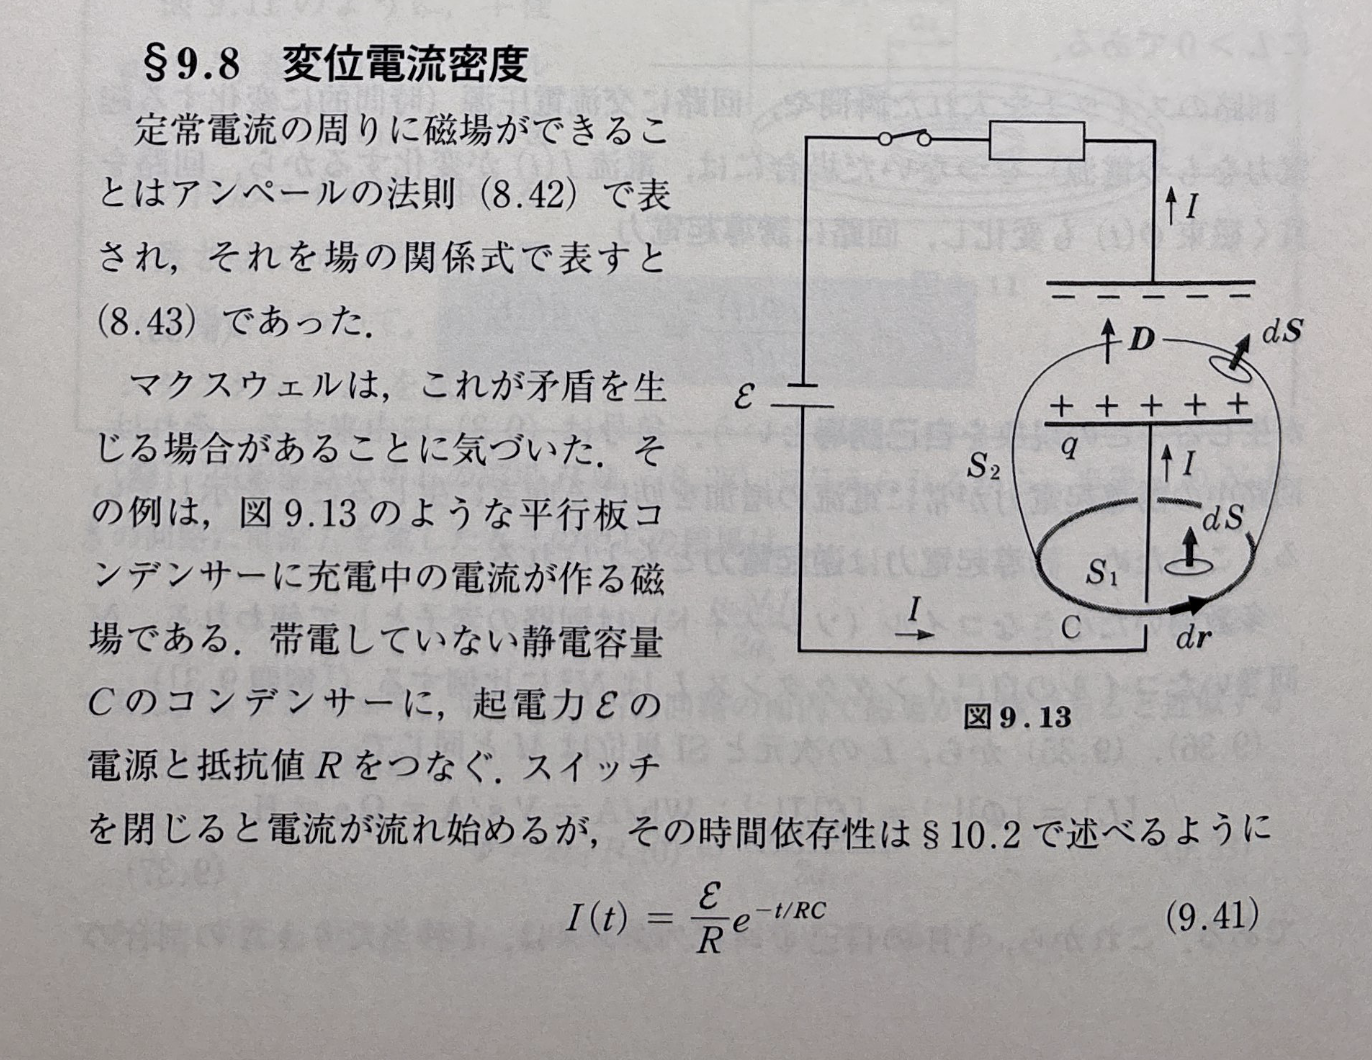
\includegraphics[width=1.0\linewidth]{images/number10.png}
\end{center}

\begin{center}
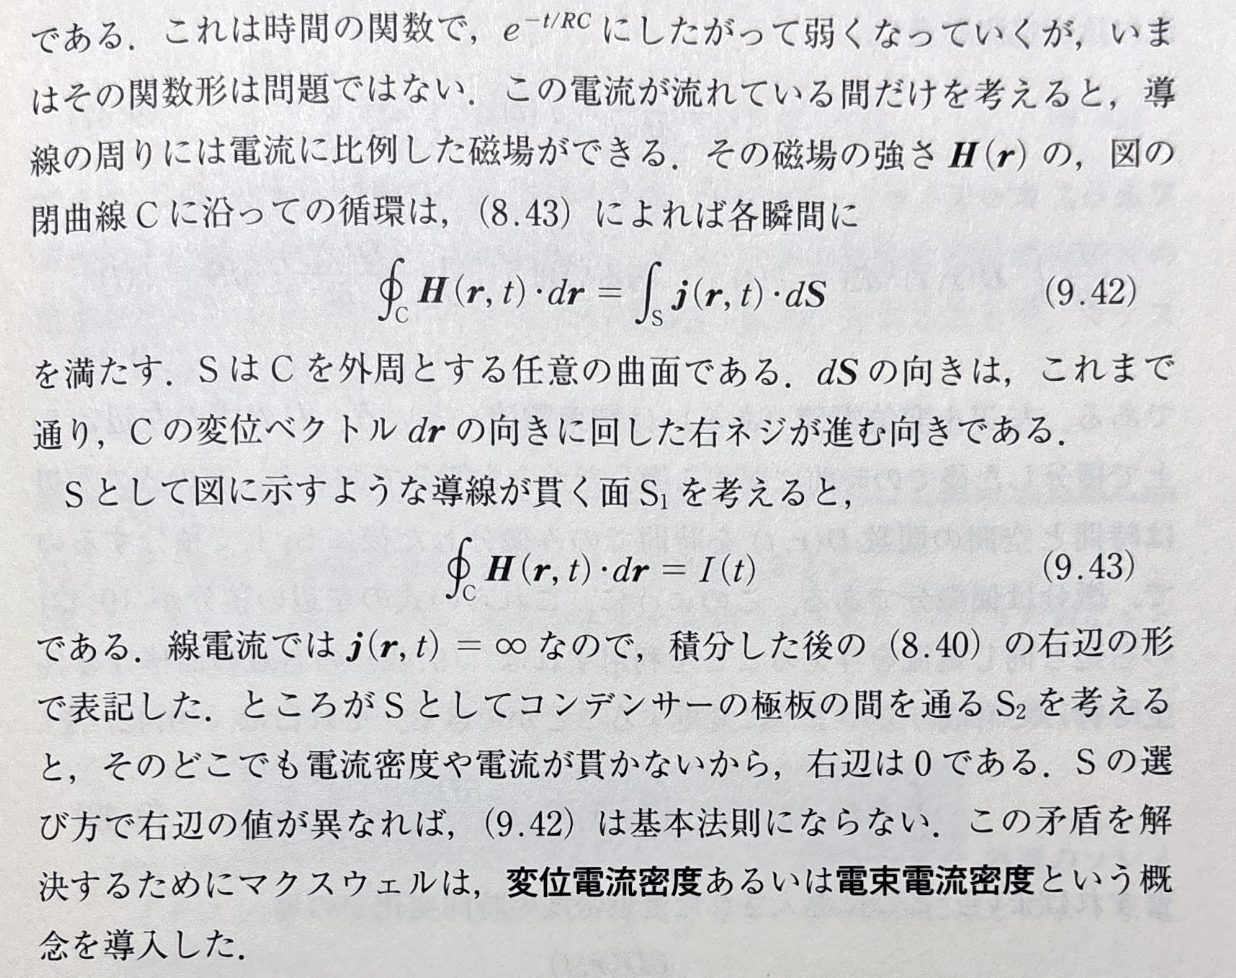
\includegraphics[width=0.9\linewidth]{images/number11.png}
\end{center}


\begin{center}
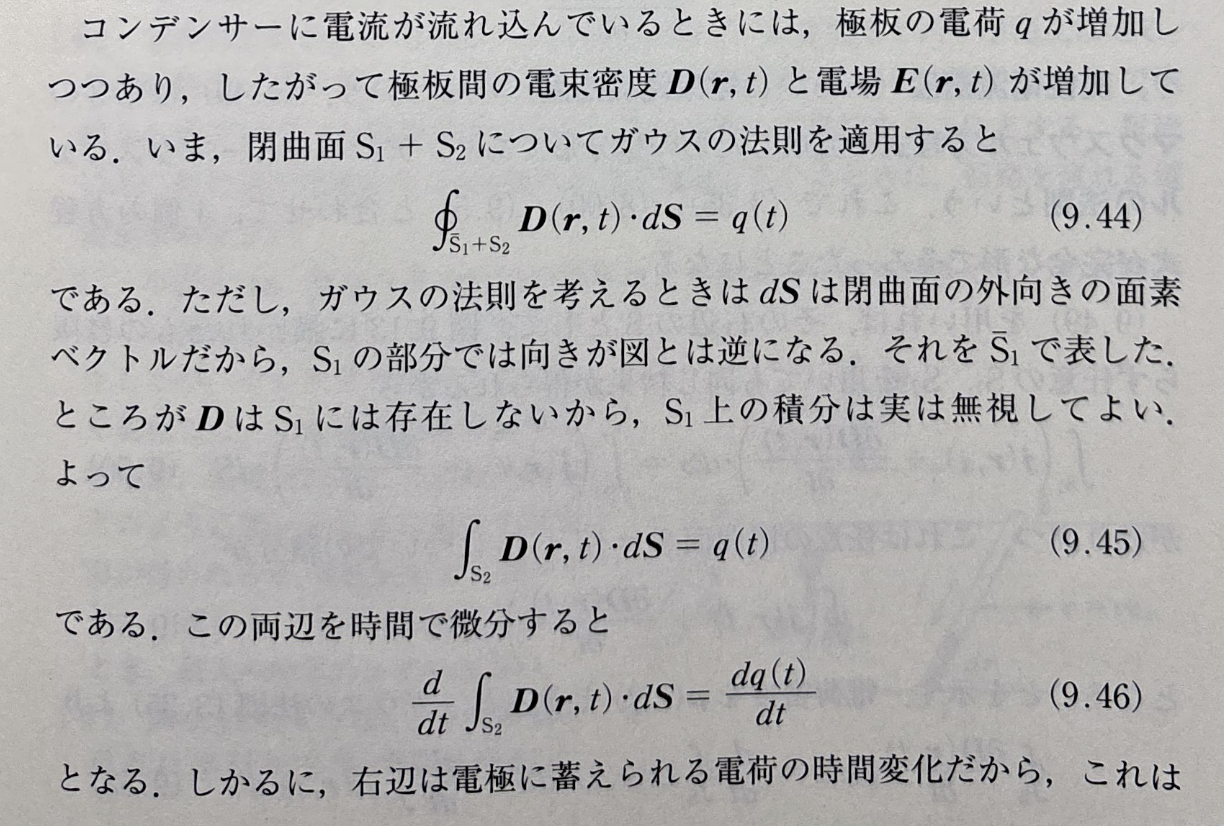
\includegraphics[width=0.9\linewidth]{images/number12.png}
\end{center}


\begin{center}
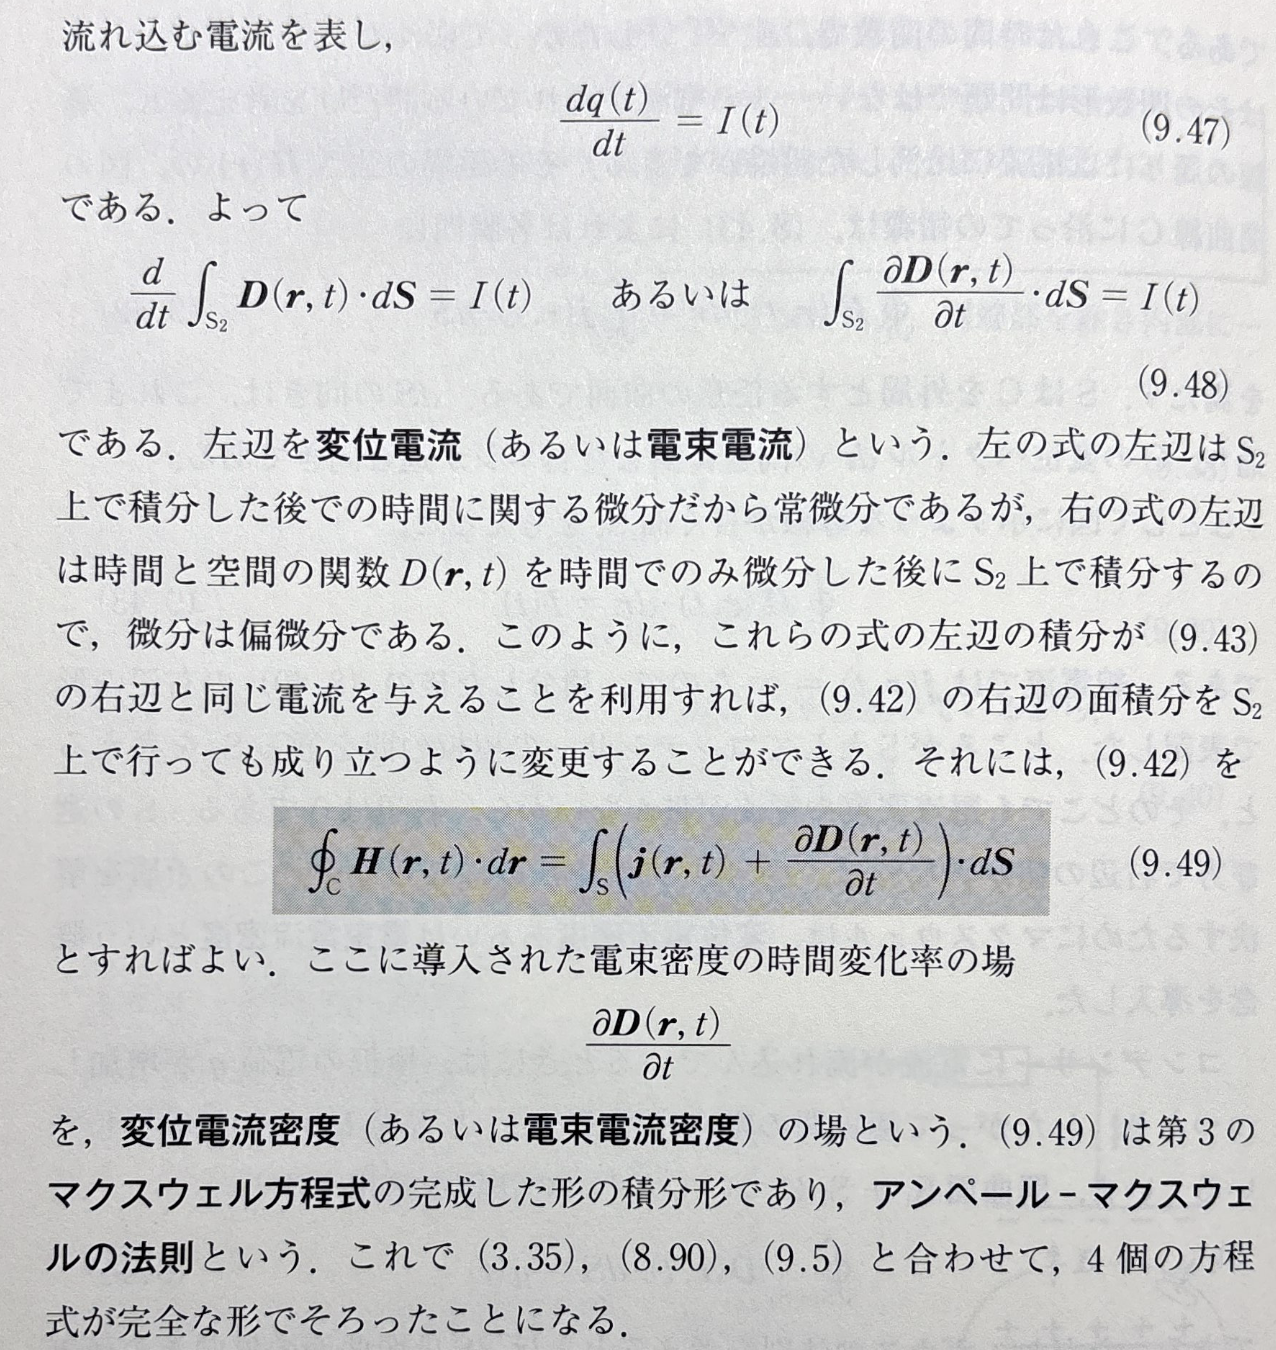
\includegraphics[width=0.8\linewidth]{images/number13.png}
\end{center}

\begin{center}
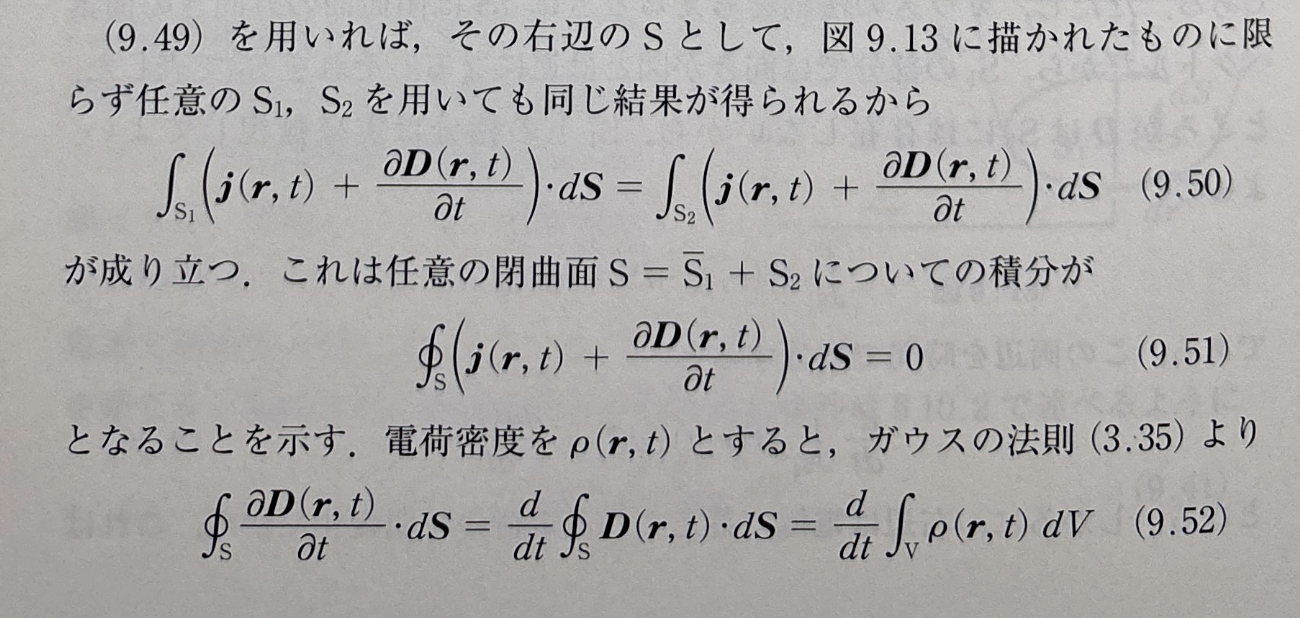
\includegraphics[width=0.9\linewidth]{images/number14.png}
\end{center}

\begin{center}
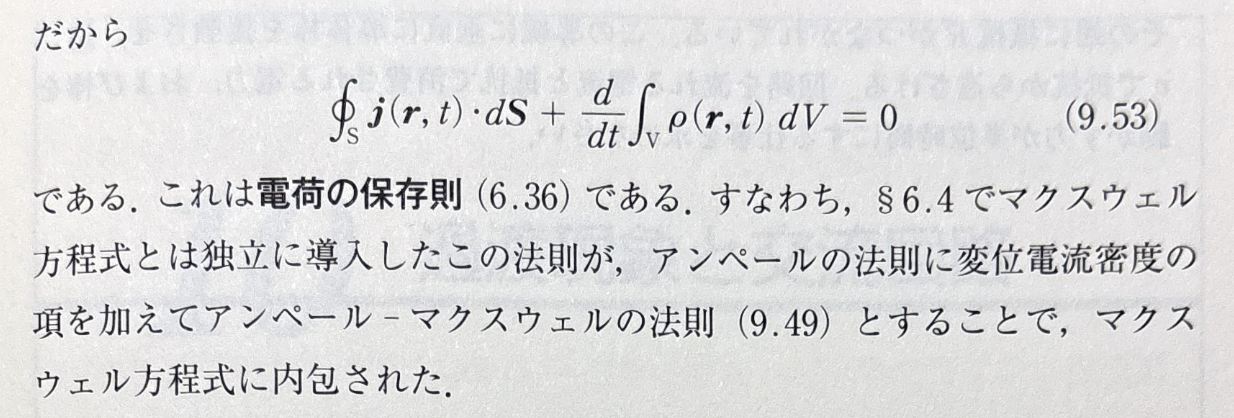
\includegraphics[width=0.9\linewidth]{images/number15.png}
\end{center}




ここで,充電したコンデンサーを考える. 

スイッチを入れると放電が起こる. 

\begin{align}
  &\text{rot} \bm{B}(\bm{r},t) - \epsilon_0 \mu_0 \frac{\partial \bm{E}(\bm{r},t)}{\partial t} = \mu_0 \bm{j}(\bm{r},t)　・・・③
\end{align}
この式の第2項がなかったら, 
\begin{align}
  &\int_{S_1}^{} \text{rot} \bm{B}(\bm{r},t)dS = \int_{S_1}^{} \mu_0 \bm{j}(\bm{r},t)dS\\
  &\int_{S_2}^{} \text{rot} \bm{B}(\bm{r},t)dS = \int_{S_2}^{} \mu_0 \bm{j}(\bm{r},t)dS
\end{align}
回路に電流が流れている間, (127)式の右辺は0でなく, (128)の左辺は0となる. 
ストークスの定理より
\begin{align}
  &①の左辺 = \int_{r}^{}\bm{B}(\bm{r},t) \cdot d\bm{r}\\
  &②の右辺 = \int_{r}^{}\bm{B}(\bm{r},t) \cdot d\bm{r} 
\end{align}
第2項がなければ(アンペールの法則), 矛盾が生じる. 
アンペールの法則に時刻$t$を入れると成り立たない. 
よって, 変位電流という考えを用いてこの問題を解決する.  

第2項がなければ
\begin{align}
  \text{rot} \bm{B}(\bm{r},t) = \mu_0 \cdot \bm{j}(\bm{r},t)
\end{align}
で両辺のdivをとると
\begin{align}
  \text{div rot} \bm{B}(\bm{r},t) = \mu_0 \text{div} \bm{j}(\bm{r},t)
\end{align}
すなわち
\begin{align}
  \text{div}\bm{j}(\bm{r},t) = 0
\end{align}
となる. 

\vspace{10mm}
\subsubsection*{電荷の保存則}

\vspace{10mm}
\begin{center}
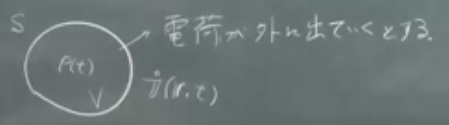
\includegraphics[width=0.8\linewidth]{images/number16.png}
\end{center}

\begin{align}
  \int_{S}^{} \bm{j}(\bm{r},t) \cdot d\bm{S} = -\frac{d}{dt} \int_{V}^{} \rho(\bm{r},t)dV
\end{align}
左辺は単位時間に$S$から出ていく電荷を表し, 右辺は$V$の内部に存在する
電荷の総量の時間微分を表す(総電荷の単位時間当たりの増加分). 

ここで,. ガウスの定理より
\begin{align}
  (左辺) = \int_{V}^{} \text{div} \bm{j}dV
\end{align}
だから
\begin{align}
  \int_{V}^{} \text{div}\bm{j}(\bm{r},t)dV = -\int_{V}^{} \rho(\bm{r},t)dV.
\end{align}
これより, 
\begin{align}
  \text{div}\bm{j}(\bm{r},t) + \frac{\partial}{\partial t}\rho(\bm{r},t) = 0.
\end{align}
これが本来成り立つべき電荷の保存則の微分形である. \par


時間依存性を考えるとアンペールの法則では不十分である. それで, これを
解決するような第2項を加えるわけである. 極板間に存在している電場(右から左)の時間変化が電流密度に相当する
ような役割を果たしているのかを考える. 右側の極板の電荷を$Q(t)$とする.
電場$E(t) = -\frac{\sigma(t)}{\epsilon_0}$($\sigma$は電荷の面密度)(右向きを正とする)
で,  $\sigma(t) = \frac{Q(t)}{A}$($A$は極板の面積)より
\begin{align}
  E(t) = -\frac{Q(t)}{\epsilon_0 A}.
\end{align}
回路に流れる電流を$I(t)$とすると
\begin{align}
  I(t) = -\frac{dQ(t)}{dt}.
\end{align}
(138)式より$Q(t) = -\epsilon_0 E(t)$を(139)式に代入して
\begin{align}
  I(t) &= -\epsilon_0 A\frac{dE(t)}{dt}\\
  \frac{I(t)}{A} &= -\epsilon_0 \frac{dE(t)}{dt}.
\end{align}

$S_1$は導線と交わっていて(電流が横切っている), $S_2$は
導線と交わっていない(電流が横切っていない). 状況として, 
両方同じように考えないとアンペールの法則の積分が成り立たねいことに
なってしまう. そこで, 極板間には
\begin{align}
  \epsilon_0 \frac{dE(t)}{dt}
\end{align}
の電流密度が保存すると考える. だから, マクスウェル方程式の③式の第2項が
出てきたのである. 

アンペールの法則
\begin{align}
  \text{rot}\bm{B} = \mu_0 \bm{j}
\end{align}
において, $\bm{j}$のかわりに$\bm{j} + \epsilon_0 \frac{\partial \bm{E}}{\partial t}$を入れると
\begin{align}
  \text{rot}\bm{B} = \mu_0 \left(\bm{j} + \epsilon_0 \frac{\partial \bm{E}}{\partial t}\right)　(マクスウェル方程式の③)
\end{align}

③で先ほどの問題が解決されるのかを確認する. 
\begin{align}
  \text{rot} \bm{B}(\bm{r},t)  =  \epsilon_0 \mu_0 \frac{\partial \bm{E}(\bm{r},t)}{\partial t} + \mu_0 \bm{j}(\bm{r},t)
\end{align}

これを$S_1, S_2$で面積分すると
\begin{align}
  &\int_{S_1}^{} \text{rot} (\bm{r},t) \cdot d\bm{S} = \int_{S_1}^{} \mu_0 \bm{j}(\bm{r},t) \cdot d\bm{S} = \mu_0 I(t)\\
  &\int_{S_2}^{} \text{rot} (\bm{r},t) \cdot d\bm{S} = \int_{S_2}^{} \epsilon_0 \mu_0\frac{\partial \bm{E}(\bm{r},t)}{\partial t} \cdot d\bm{S} = -\mu_0 \frac{Q(t)}{dt}
\end{align}
マクスウェル方程式③のdivを計算して
\begin{align}
  \text{div rot}\bm{B} - \epsilon_0 \mu_0 \text{div} \frac{\partial \bm{E}}{\partial t} = \mu_0 \text{div} \bm{j} (\bm{r},t).
\end{align}
$\text{div}\bm{E} = \frac{\rho}{\epsilon_0}$だから(ガウスの法則)

\begin{align}
  &\frac{\partial \rho}{\partial t} + \text{div}\bm{j} = 0\\
  &\frac{\partial \rho(\bm{r},t)}{\partial t} + \text{div}\bm{j}(\bm{r},t) = 0
\end{align}
よって, 電極の周りの面積分で起こる矛盾は解決されて, 
電荷の保存則が成り立つことがわかった. 
また, (142)は変位電流密度という.


この項が電磁波につながってくる. 




\newpage

\subsection*{マクスウェル方程式とファラデー(電磁誘導)の法則}
磁束とは磁束密度を面積分すれば良い. 

\begin{align}
  \Phi(t) = \int_{S}^{} \bm{B}(\bm{r},t) \cdot d\bm{S}
\end{align}

\begin{center}

\includegraphics[width=0.3\linewidth]{images/number8.png}
\end{center}

ファラデーの法則は
\begin{align}
  -\frac{d\Phi(t)}{dt} &= \oint_{C}^{} \bm{E}(\bm{r},t) \cdot d\bm{r}　\\
  (誘導起電力) &= (誘導電場)
\end{align}
\begin{align}
  -\frac{d}{dt} \int_{S}^{} \bm{B}(\bm{r},t) \cdot d\bm{S} &= \oint_{C}^{} \bm{E}(\bm{r},t) \cdot d\bm{r}\\
  &= \int_{S}^{} \text{rot} \bm{E}(\bm{r},t) \cdot d\bm{S}
\end{align}

\begin{align}
  &\int_{S}^{} \text{rot} \bm{E}(\bm{r},t)d\bm{S} + \int_{S}^{} \frac{\partial \bm{B}(\bm{r},t)}{\partial t} \cdot d\bm{S} = 0\\
  &\int_{S}^{} \left(\text{rot}(\bm{r},t) + \frac{\partial \bm{B}(\bm{r},t)}{\partial t}\right)\cdot d\bm{S} = 0
\end{align}
したがって, 
\begin{align}
  \text{rot}(\bm{r},t) + \frac{\partial \bm{B}(\bm{r},t)}{\partial t} = 0
\end{align}
となり, 
\begin{align}
  &\text{rot} \bm{E}(\bm{r},t) + \frac{\partial \bm{B}(\bm{r},t)}{\partial t} = 0　・・・②
\end{align}
が導出された. その逆も辿れる. ②式は微分形のファラデーの法則に他ならない. 





\newpage

\subsection*{磁束密度に対するガウスの法則}
\begin{align}
  \int_{S}^{} \bm{B}(\bm{r},t) \cdot d\bm{S} = 0
\end{align}
単磁極が存在しないから0.


\begin{center}

\includegraphics[width=0.3\linewidth]{images/number9.png}
\end{center}

ガウスの法則を使って,
\begin{align}
  \int_{V}^{} \text{div} \bm{B}(\bm{r},t)dV.
\end{align}
これが任意の$V$に対して成り立つので, 
\begin{align}
  \text{div}\bm{B}(\bm{r},t) = 0
\end{align}
となり, ④式が成り立つ. 




\newpage

\section*{ポアソン方程式,ラプラス方程式}

マクスウェル方程式の第一式
\begin{align}
  \text{div} \bm{E}(\bm{r},t) = \frac{\rho(\bm{r},t)}{\epsilon_0}
\end{align}
に
\begin{align}
  \bm{E}(\bm{r},t) = -\text{grad}\phi(\bm{r},t) 
\end{align}
を代入すると
\begin{align}
  &\text{div grad} \phi(\bm{r},t) = -\frac{\rho(\bm{r},t)}{\epsilon_0}\\
  &\laplacian{\phi(\bm{r},t)} = -\frac{\rho(\bm{r},t)}{\epsilon_0}
\end{align}
これをポアソン方程式という.
$\rho(\bm{r},t) = 0$のときは
\begin{align}
  \laplacian{\phi(\bm{r},t)} = 0.
\end{align}
これをラプラス方程式という. 




\newpage
\section*{電磁波}





\end{document}
